\problemname{Bingo Boards
}

John loves Bingo! At his local pub, they play a special version of Bingo every Thursday called Big Bingo.

In Big Bingo, you have an $N \times N$ grid of numbers. Each number from 1 to $N^2$ appears exactly once in the grid. The host of the event calls out numbers one at a time, and for each one, you mark the cell containing it. Your board wins if every cell in some row or some column is marked. Unlike normal Bingo, you cannot win with diagonals.

Things are getting very exciting this week: as John looks down, he realizes that no matter which of the five remaining numbers are called, he will win.

\begin{center}
 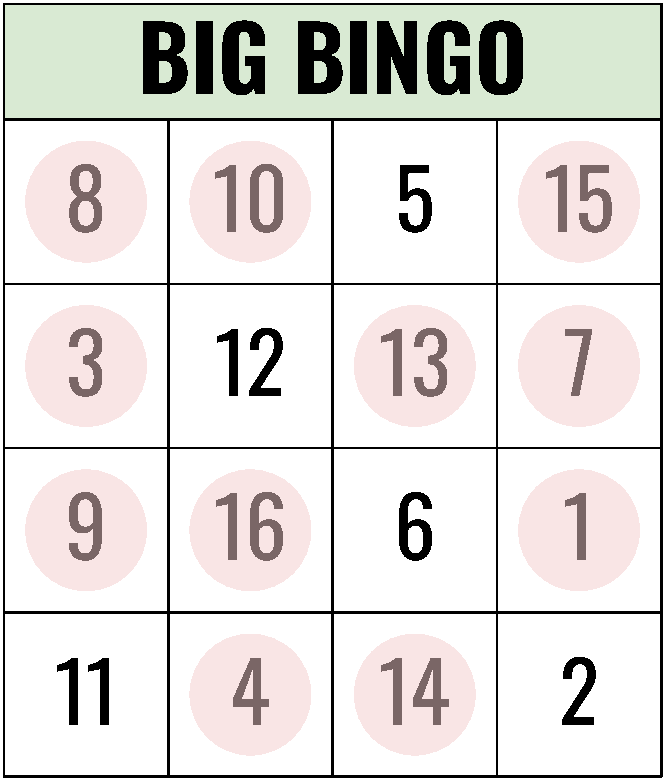
\includegraphics[width=0.5\textwidth]{BigBingo}
\end{center}

A partially marked board is \textit{on the verge} if (1) it is not a winning board based on the already marked numbers and (2) marking any of the unmarked numbers will make it a winning board.

John wonders how common this is. Given $N$ and $k$, find an $N \times N$ board that has exactly $k$ marked cells and is on the verge, or state that one doesn't exist.



\section*{Input}

The input consists of a single line containing two integers $N$~($1 \leq N \leq 200$), which is the size of the board, and $k$~($0 \leq k \leq N^2$), which is the desired number of marked cells.


\section*{Output}

If it is impossible to construct a $N \times N$ board containing $k$ marked cells that is also on the verge, display \texttt{IMPOSSIBLE}.

Otherwise, display \texttt{POSSIBLE}, then display a valid board showing such a marking. The board must be an $N \times N$ grid of dots (`\texttt{.}') and hashes (`\texttt{\#}') without any spaces separating characters on the same line. The $j$th character of the $i$th row denotes whether the cell $(i, j)$ is marked (\texttt{\#}) or not (\texttt{.}).

If there are multiple valid solutions, any will be accepted.
